\documentclass[tikz,border=2pt]{standalone}
\usepackage{amsmath,amssymb}
\usepackage{tikz}

\begin{document}
% Independence as areas: in the unit square, A is a vertical band of width P(A) and B a
% horizontal band of height P(B); their overlap has area P(A) P(B), so knowing B does not
% change the share of A.
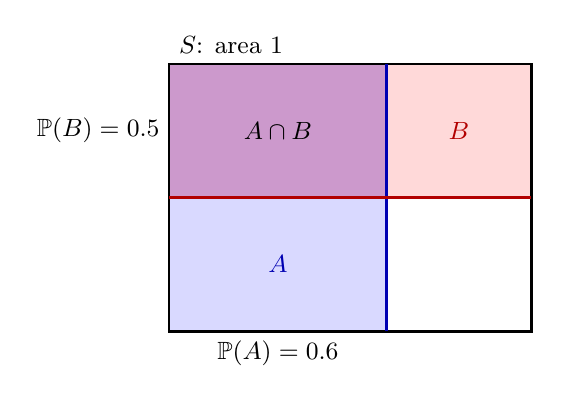
\begin{tikzpicture}[every node/.style={font=\small}, x=4.6cm, y=3.4cm]
	\fill[blue!15] (0,0) rectangle (0.6,1);
	\fill[red!15] (0,0.5) rectangle (1,1);
	\fill[violet!40] (0,0.5) rectangle (0.6,1);
	\draw[thick] (0,0) rectangle (1,1);
	\draw[thick, blue!70!black] (0.6,0) -- (0.6,1);
	\draw[thick, red!70!black] (0,0.5) -- (1,0.5);
	\node[blue!70!black] at (0.3,0.25) {$A$};
	\node[red!70!black] at (0.8,0.75) {$B$};
	\node at (0.3,0.75) {$A\cap B$};
	\node[below, font=\small] at (0.3,0) {$\mathbb{P}(A)=0.6$};
	\node[left, font=\small] at (0,0.75) {$\mathbb{P}(B)=0.5$};
	\node[anchor=south west] at (0,1.0) {$S$: area $1$};
	
\end{tikzpicture}
\end{document}
